\documentclass[AMA,STIX1COL]{WileyNJD-v2}\usepackage[]{graphicx}\usepackage[]{color}
%% maxwidth is the original width if it is less than linewidth
%% otherwise use linewidth (to make sure the graphics do not exceed the margin)
\makeatletter
\def\maxwidth{ %
  \ifdim\Gin@nat@width>\linewidth
    \linewidth
  \else
    \Gin@nat@width
  \fi
}
\makeatother

\definecolor{fgcolor}{rgb}{0.345, 0.345, 0.345}
\newcommand{\hlnum}[1]{\textcolor[rgb]{0.686,0.059,0.569}{#1}}%
\newcommand{\hlstr}[1]{\textcolor[rgb]{0.192,0.494,0.8}{#1}}%
\newcommand{\hlcom}[1]{\textcolor[rgb]{0.678,0.584,0.686}{\textit{#1}}}%
\newcommand{\hlopt}[1]{\textcolor[rgb]{0,0,0}{#1}}%
\newcommand{\hlstd}[1]{\textcolor[rgb]{0.345,0.345,0.345}{#1}}%
\newcommand{\hlkwa}[1]{\textcolor[rgb]{0.161,0.373,0.58}{\textbf{#1}}}%
\newcommand{\hlkwb}[1]{\textcolor[rgb]{0.69,0.353,0.396}{#1}}%
\newcommand{\hlkwc}[1]{\textcolor[rgb]{0.333,0.667,0.333}{#1}}%
\newcommand{\hlkwd}[1]{\textcolor[rgb]{0.737,0.353,0.396}{\textbf{#1}}}%
\let\hlipl\hlkwb

\usepackage{framed}
\makeatletter
\newenvironment{kframe}{%
 \def\at@end@of@kframe{}%
 \ifinner\ifhmode%
  \def\at@end@of@kframe{\end{minipage}}%
  \begin{minipage}{\columnwidth}%
 \fi\fi%
 \def\FrameCommand##1{\hskip\@totalleftmargin \hskip-\fboxsep
 \colorbox{shadecolor}{##1}\hskip-\fboxsep
     % There is no \\@totalrightmargin, so:
     \hskip-\linewidth \hskip-\@totalleftmargin \hskip\columnwidth}%
 \MakeFramed {\advance\hsize-\width
   \@totalleftmargin\z@ \linewidth\hsize
   \@setminipage}}%
 {\par\unskip\endMakeFramed%
 \at@end@of@kframe}
\makeatother

\definecolor{shadecolor}{rgb}{.97, .97, .97}
\definecolor{messagecolor}{rgb}{0, 0, 0}
\definecolor{warningcolor}{rgb}{1, 0, 1}
\definecolor{errorcolor}{rgb}{1, 0, 0}
\newenvironment{knitrout}{}{} % an empty environment to be redefined in TeX

\usepackage{alltt}

\articletype{Research Article}%???

\received{26 April 2016}
\revised{6 June 2016}
\accepted{6 June 2016}

\raggedbottom
\IfFileExists{upquote.sty}{\usepackage{upquote}}{}
\begin{document}

\title{Bayesian Reproducibility %\protect\thanks{This is an example for title footnote.}
}

\author[1]{Huijia Yu}

\author[2]{Merlise Clyde*}


\authormark{HUIJIA YU \textsc{et al}}


\address[1]{\orgdiv{Department of Statistical Science}, \orgname{Duke University}, \orgaddress{\state{North Carolina}, \country{USA}}}
\address[2]{\orgdiv{Department of Statistical Science}, \orgname{Duke University}, \orgaddress{\state{North Carolina}, \country{USA}}}


\corres{*Merlise Clyde, Department of Statistical Science, Duke University, Durham, North Carolina, USA. \email{clyde@duke.edu}}

\abstract[Summary]{
Parameter estimates from initial discovery data in genome-wide association studies (GWAS) often have upward bias compared to subsequent validation studies, which are underpowered due to the inflated effect estimate. This effect, known as the winner's curse, can be attributed to the double use of data, which must first pass a significance test. We propose three Bayesian approaches to discovery reporting and validation analysis: a fully Bayesian hierarchical model with a spike and slab prior, a conditional likelihood approach that only requires sufficient statistics from the discovery data, and an empirical approximation for the spike and slab prior using a Bayes factor approximation of the discovery data. We examine these methods with simulation studies and a real data example. All three proposed methods perform better than a naive models in the simulation studies, and produce results congruent with recent findings in the real example.

}

\keywords{p value, bayes factor,winner's curse, hierarchical Bayes model, meta-analysis}

\jnlcitation{\cname{ %this is the citation for this article!
\author{Yu H.}, 
\author{Clyde M,}} (\cyear{2018}), 
\ctitle{Bayesian Reproducibility}, \cjournal{Q.J.R. Meteorol. Soc.}, \cvol{2017;00:1--6}.} %????

\maketitle

% \footnotetext{\textbf{Abbreviations:} ANA, anti-nuclear antibodies; APC, antigen-presenting cells; IRF, interferon regulatory factor} this is a title footnote






\section{Introduction}\label{sec:intro}

P-values have been on of the reasons behind lack of reproducibility in scientific discoveries and especially in replicated studies and multiple testing\cite{benjamin2017redefine}. This problem is especially prevalent in Genome-Wide Association Studies (GWAS), where estimated effects have upward bias and often fail to replicate in validation studies. This phenomenon is known as the winner's curse  \cite{zollner2007overcoming}. To account for this discrepancy, previous studies perform two analyses: one with all the data together, and one only using the validation site data. However, this approach is based on the underlying assumption that the association found in discovery sites is true, which is problematic for multiple testing applications such as genome-wide association studies. Furthermore, if there is a true effect, leaving out the discovery data, which could be a large portion of the total dataset, reduces power.

One example of the winner's curse in action is the analysis of the association between single nucleotide polymorphisms (SNPs) in the p53 protein, which is needed for cell growth and DNA repair, and invasive ovarian cancer. Three independent discovery studies focused on TP53 polymorphisms and risk of ovarian cancer: the North Carolina Ovarian Cancer Study (NCOCS), the Mayo Clinic Case-Control Study (MAYO), and the Polish Ovarian Cancer Study (POCS). These were restricted to non-Hispanic white women with newly diagnosed, histologically confirmed, primary invasive epithelial ovarian cancer and to non-Hispanic white controls. 23 SNPs were genotyped in total, with some overlap between sites. Ten other sites contributed data: the Australian Ovarian Cancer Study (AOCS) and the Australian Cancer Study (ACS) presented together as AUS, the Family Registry for Ovarian Cancer (FROC, presented as STA), the Hawaiian Ovarian Cancer Study (HAW), the Malignant Ovarian Cancer Study Denmark (MALOVA), the New England Case-Control Study (NEC), the Nurses' Health Study (NHS), SEARCH Cambridge (SEA), the Los Angeles County Case-Control Study of Ovarian Cancer (LAC-CCOC, presented here as USC), the University of California at Irvine study (UCI), and the United Kingdom Ovarian Cancer Population Study (UKOPS, presented here as UKO). The combined data set (discovery and replication) comprised 5,206 white, non-Hispanic invasive epithelial ovarian cancer cases, of which 2,829 were classified as serous invasive ovarian cancer, and 8,790 white non-Hispanic controls. Analysis was restricted to white, non-Hispanic invasive serous ovarian cancer cases and white, non-Hispanic controls.

Mixed effect SNP-at-a-time analysis of 5 SNPs that were chosen for replication resulted in associations between 2 SNPs and serous invasive cancer \cite{Schildkraut2349}. Only one of these was strongly supported to be associated in a follow-up analysis using Multi-level Inference for SNP Association (MISA), which employs Bayesian Model Averaging and Bayes Factors for selection \cite{schildkraut2010association}. However, most recent studies with added data have not found evidence of association between any TP53 SNPs and cancer \cite{phelan2017identification}.

The aim of this project is twofold: to explore ways in which discovery findings can be reported to avoid the winner's curse, and to combine discovery results with validation data in a coherent manner accounting for the selection effect. 

After a review of existing literature, we propose three approaches to adress this: a fully Bayesian model, a conditional likelihood prior for discovery site data, and a Bayes Factor approximation to the probability of association. The performance of these methods is tested on normal simulations, and then on hierarchical simulations split into discovery and validation "sites". All three proposed methods provide improvements over naive models. Finally, the models are used to reanalyze the tp53 SNPs; only one of them is found to be significant.

\section{Literature Review}\label{sec:lit}

Misuse of p-values and lack of reproducibility in scientific discoveries have been a cause for concern in the scientic world, leading to proposals of new ways to define significance. Benjamin et. al have shown that the Bayes factor equivalents for commonly used p-values only correspond to "weak" evidence in the Bayes factor characterization \cite{benjamin2017redefine}. They suggest reducing the p-value threshold in studies with less power, but acknowledge that hypothesis testing with thresholding is still an issue. Another approach proposes two calibrations of the p-value: as the lower bound of the Bayes factor under any alternative hypothesis, and as a posterior probability of the type 1 error in a Bayesian framework \cite{sellke2001calibration}.

This problem has become a major issue in replicated studies, an effect known as the "winner's curse" \cite{zollner2007overcoming} or the Beavis effect \cite{xu2003theoretical}. Zollner and Pritchard first define this in the context of genome-wide association scans (GWAS), which use stringent thresholds for significance, resulting in inflated effect sizes after selection, especially since these are calculated with the same data. Thus, replication studies underestimate the sample size necessary and do not have enough power to detect an effect. They suggest a conditional-likelihood based method to address this issue, proposing a computational algorithm to maximize over the the likelihood of the parameters conditional on the significance association at level $\alpha$, which results in less biased coefficient estimates (albeit with larger variance) and sample size estimates centered at the true value \cite{zollner2007overcoming}.

Zhong and Prentice also propose a similar method, but use a different parametrization and an asymptotic approximation instead of a computational one to find the estimators, which is more computationally efficient \cite{zhong2008bias}. Ghosh et al. also define an approximate conditional likelihood, and propose two more estimators (other than the MLE): the mean of the (normalized) conditional likelihood, which can be interpreted as a posterior mean of the parameters under a flat prior, and a "compromise" estimator which is the average of the mean and MLE \cite{ghosh2008estimating}. The combination estimator proves to have the most stable MSE accross the range of true values for the parameters. Their approach only requires summary statistics, so they further apply it to published datasets. The results are similar for the three conditional likelihood approaches.

Another method proposed to create bias-reduced estimates uses bootstrap re-sampling to correct for both the thresholding effect and the ranking effect, which is not addressed in the conditional likelihood methods because of the difficulty of specifying joint likelihoods for correlated variables \cite{sun2011br}. By using a sample-split approach, the detection and estimation datasets can be virtually independent. This is repeated multiple times in order to reduce variance in the results. The main drawback of this approach is its computational intensity.

Several authors have also proposed shrinkage-based methods in the effect detection step. Bacanu and Kendler use a soft threshold method to scale statistics such that their sum of squares do not overestimate the true mean and then find "suggestive" signals in a GWAS context by setting a threshold. This method does not address the winner's curse directly, but provides a subset of the genome which can be futher analyzed or used in future studies \cite{bacanu2013extracting}. Bigdelli et al. propose shrinking coefficient estimates by drawing a comparison between "winner's curse adjustments" for effect sizes and multiple testing approaches for p-values, since both are used on the tail of their respective distributions. Their method transforms False Discovery Rate (FDR) adjusted p-values into the corresponding Z-score and uses that as the estimator \cite{bigdeli2016simple}. Both Bigdelli and Bacanu assume the data is normally distributed. Storey and Tibshirani, on the other hand, propose to adjust the value used for significance testing rather than the coefficients, choosing the FDR value as an alternative to the p-valu e\cite{storey2003statistical}.

Multiple Bayesian methods have also been proposed: Xu et al use a Bayesian approach to a logistic regression, selecting a spike and slab prior for the mean and an inverse gamma prior for the variance \cite{xu2011bayesian}. A beta prior for the proportion of each component in the prior, and the hyperparameters were estimated empirically. They also propose a Bayesian Model Average approach, which they recommend for instances with little prior information. Their results show that the Bayesian models had smaller variance than conditional likelihood methods, but still do not address the "ranking effect" \cite{sun2011br}, or implement a fully Bayesian approach because of the dependence on the threshold $\alpha$.

Ferguson et al propose an Empirical Bayes approach, which estimate the prior density distribution with the data \cite{ferguson2013empirical}. This is a nonparametric estimate, but still depends on other specifications such as the number of bins, type of splines, etc. Using the empirical prior, the posterior is then calculated, from which the estimate and pseudo-Bayesian credible intervals are derived by considering the 5\% and 95\% points. This method resulted in better estimates in the higher density regions, but performed worse than conditional likelihood methods on the tails. Thus, the authors propose a combined method, which calculates both the empirical Bayes and the conditional likelihood confidence intervals, and picks the shortest one. One possible problem with this approach is the use of non-HPD intervals, which could change the tail behavior.

The Bayesian framework is also applied to power calculations specifically, defining "Bayesian power" as the marginal probability of finding significance in a replicated study given the original and the data. In this paper, a spike and slab prior is also used, but the hyperparameters are estimated empirically. The resulting power estimators are improved, but lead to downwards bias in the effect size \cite{jiang2016power}.

\section{Models}\label{sec:models}


Following the structure of the motivating example, consider a binary dataset describing an event such as whether or not someone has ovarian cancer. This data is collected across different sites, which may have different sampling procedures (as well as simply different populations). The mean effect for each site can be thought of as normally distributed around a global effect if this exists. This is the alternative hypothesis. The null hypothesis is that there is no global effect. This also means that there must not be a site effect. We are interested in two things: whether or not there is a global effect (hypothesis testing), and what the effect's size is (inference). Let $Y_{ij}$ be the observed data. The $j$ index corresponds to the site to which the observation belongs. 

\begin{gather}\label{eq1}
P(Y_{ij}=1| \beta_j) = \textsf{logit}^{-1}(\beta_{j})\\
\beta_{j}|\mu, \sigma^2,H_1 \sim \textsf{N}(\mu, \sigma^{2})\\
\beta_{j}|H_0 = 0
\end{gather}

In the case where we have multiple sites' information, we can use this hierarchical model, but if we only have data from one discovery site, then the site effect becomes meaningless, and we can use the following model:

\begin{equation}\label{eq2}
P(Y_{i}=1|\mu) = \textsf{logit}^{-1}(\mu)
\end{equation}

We propose three different Bayesian approaches: 

1. A fully Bayesian mixed effects hierarchical model that can jointly perform significance testing and effect estimation. By combining the testing and estimate steps, we can overcome the winner's curse and account for the uncertainty that arises when selecting an SNP. This model builds on Xu et al. \cite{xu2011bayesian}, and Jiang et al. \cite{jiang2016power}, which introduce the spike-and-slab prior, with the addition of random effects to account for heterogeneity between sites.

2. A conditional likelihood model that can take into account the probability of finding a significant result in the discovery sites when estimating effect size. This model incorporates the conditional likelihood introduced by Zollner and Pritchard as well as Zhong and Prentice, and Ghosh et al.)\cite{zollner2007overcoming, zhong2008bias, ghosh2008estimating} and incorporates it into the Bayesian hierarchical framework.

3. A Bayes factor-based model that uses an upper bound on the Bayes factor from the discovery sites, which is more reliable than the p-value \cite{benjamin2017redefine} to quantify the uncertainty of the significant result.

While the first approach is truly Bayesian and requires all the data, the second and third can be used as long as the sufficient statistics (MLE, SE, p-value, $\alpha$) are available. 


\subsection{Fully Bayesian Model}

Let $\delta_a(x)$ be the Dirac delta function: $\delta_a(x) = 1$ for $x = a$ and $\delta_a(x)=0$ otherwise. Then, $P( \mu|H_0) = \delta_0 ( \mu )$,  and $P( \mu|H_1) = N(0,1)$ or some other diffuse prior. We can define a hyperparameter $\xi$ such that $P(H_1) = \xi$. This gives rise to a latent variable drawn from a Bernoulli($\xi$), which is equivalent to selecting $H_1$ or $H_0$. Site means $\beta_{j}|\mu, \sigma^2,H_1 \sim N(\mu, \sigma^2)$, and $\beta_{j}|H_0 = 0$. In this case the prior for  $\mu| H_1$ was chosen to be a Cauchy distribution. The prior for $\sigma$ was a truncated Cauchy, with support only on the positive real line. The prior for $\xi$, the probability of the alternative, was a Beta distribution.  The complete model is as follows:

\begin{gather}\label{eq3}
\beta_{j}|H_ 1 \sim \textsf{N}(\mu, \sigma_{\beta}^{2}) \\
\mu|H_1\sim \textsf{Cauchy}(0,\sigma_{\mu}^{2})\\
\mu, \beta_{j}|H_0  =0\\
\sigma_{\beta}\sim \textsf{Cauchy}^+(0,\sigma_{\sigma}^{2})\\
H\sim \textsf{Bernoulli}(\xi)\\
\xi \sim \textsf{Beta}(a, b)
\end{gather}

\begin{knitrout}
\definecolor{shadecolor}{rgb}{0.969, 0.969, 0.969}\color{fgcolor}

{\centering 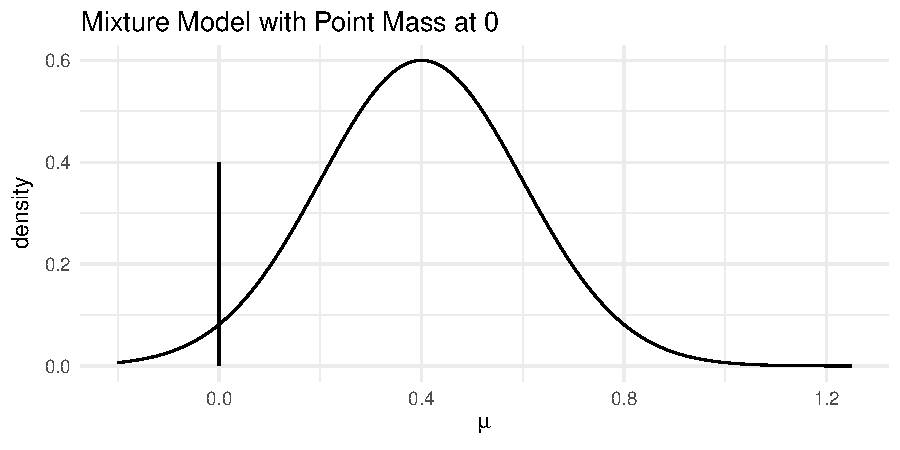
\includegraphics[width=4in]{figure/mixture-1} 

}



\end{knitrout}


If we only consider discovery data from one site, this model becomes the same as the one proposed by Xu et al. with slightly different priors. There is no difference between discovery and validation sites in the Bayesian framework. Even considering them separately, one could consider the posterior distributions of the parameters given only discovery site data as the priors given the validation data, which would result in exactly the same results. 

\subsection{Conditional Likelihood Model}

In this case, the results from the discovery sites are used as a prior for the validation data analysis, which is why only the sufficient statistics are needed. Given the discovery sites' MLE and SE, we can use the CLT and definition of MLE to state that $\text{MLE}_i \sim N(\beta_i, \text{SE}_i)$. Let $B$ indicate that the data is significant at the level $\alpha$. The conditional likelihood is:

\begin{equation}\label{eq4}
L(\mu | B) = \frac{p(Y| \mu)p(B| Y,\mu)}{p(B|\mu)} =  \frac{p(Y| \mu)}{\int_{\textsf{significant Y}} p(t| \mu) dt }
\end{equation}

Conditioning on finding a significant estimate using a Normal approximation, 

\begin{equation}\label{eq5}
p(\text{MLE}_i | B,\beta_i,\text{SE}_i,q_i) = \frac{\phi(\text{MLE}_i, \beta_i, \text{SE}_i)}{\Phi(-q_i, \beta_i, \text{SE}_i)+1-\Phi(q_i, \beta_i, \text{SE}_i)}
\end{equation}

where $\phi(x, \beta_i, \sigma)$ is the pdf of a normal distribution with mean $\beta_i$ and variance $\sigma^2$, and $\Phi(x, \beta_i, \sigma)$ is the cdf of the same distribution. The value of $q_i$ is $\Phi^{-1}(1-\frac{\alpha}{2}, 0 ,\text{SE}_i)$, where $\alpha$ is the power of the test (i.e. p-values that are smaller than $\alpha$ are considered significant). This is cutoff for an MLE value to be considered significant. Let the conditional likelihood of $\text{MLE}_i$  be denoted as $\textsf{CL}(\beta_i,\text{SE}_i, q_i)$.




\begin{figure}
\begin{knitrout}
\definecolor{shadecolor}{rgb}{0.969, 0.969, 0.969}\color{fgcolor}

{\centering 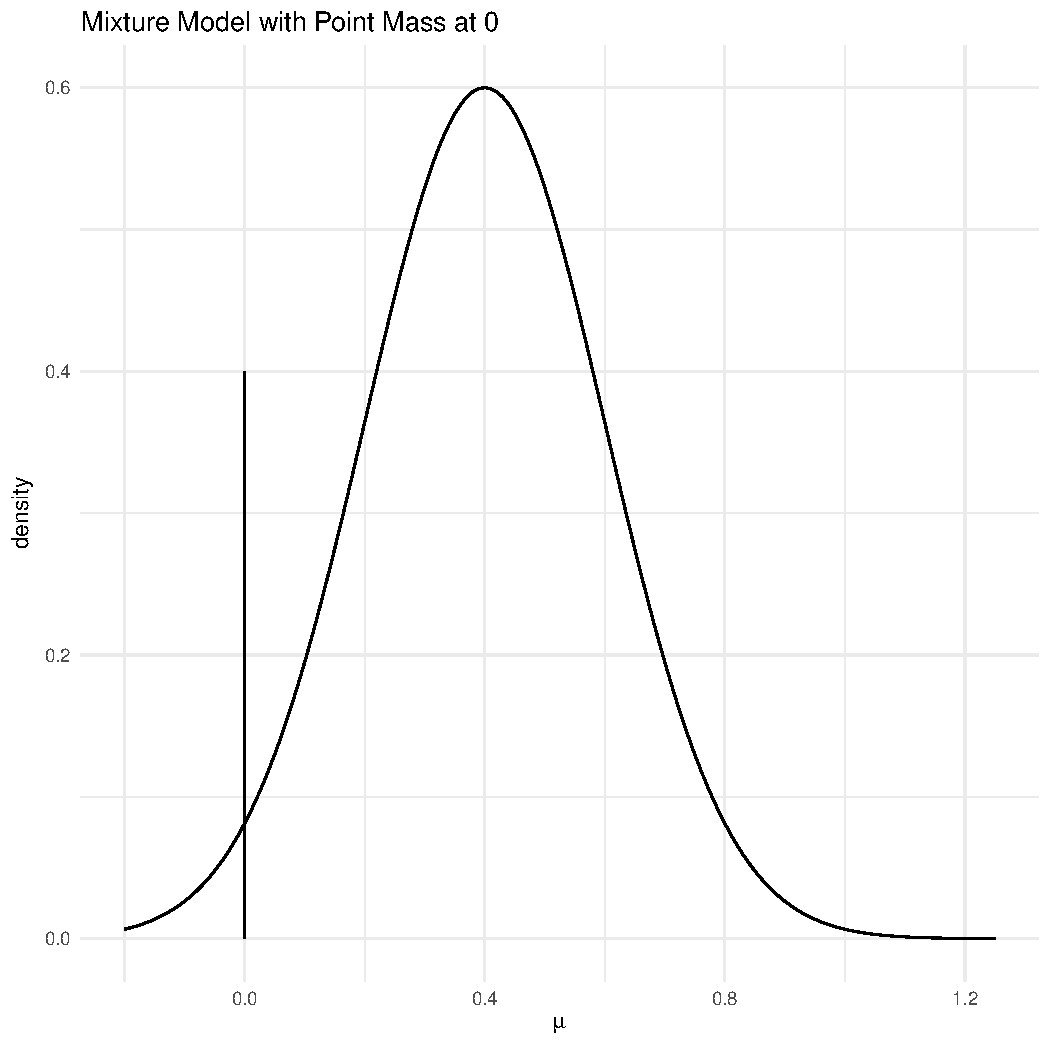
\includegraphics[width=4in]{figure/unnamed-chunk-3-1} 

}



\end{knitrout}
\end{figure}
We can see that as $\alpha$ decreases (i.e. the tests are more strict), the likelihood becomes more skewed towards 0. The conditional likelihood of $\beta_{ j}, j\in \text{discovery}$ becomes the posterior of this variable if we use a uniform prior, since the likelihood will just be multiplied by one. In the discovery-only case, this is enough to create credible intervals for $\mu$ by sampling from the posterior (as opposed to maximizing the conditional likelihood or approximating the surface).


In the hierarchical setting, the posteriors for the discovery sites are used as the priors for the validation data; that is, $p(\mu| \beta_i, \text{MLE}_i,\text{SE}_i, q_i, i \in  \text{discovery})$ is the prior for the hierarchical model using validation data. The updated model is:

\begin{gather} \label{eq6}
\beta_{j}|\mu, \sigma_{\beta}^{2} \sim \textsf{N}(\mu, \sigma_{\beta}^{2}) , j \in \text{validation}\\
\text{MLE}_{j}|\beta_{j},\text{SE}_{j}, q_j \sim \textsf{CL}(\beta_{j},\text{SE}_{j}, q_j) , j \in \text{discovery}\\
\sigma_{\beta}\sim \textsf{Cauchy}^+(0,\sigma^2_{\sigma})
\end{gather}

Note that the selection uncertainty is somewhat accounted for through the conditional likelihood, but there is no measure of this uncertainty. By using the discovery MLEs, we are already assuming that there is a nonzero effect.


\subsection{Bayes Factor Model}

The discovery data can be used not only in estimating the distribution of the size of a preestablished effect ($\mu$), but in estimating the distribution of the probability of the effect itself ($\xi = P(H_1)$). To make this model easily generalizable, we use the upper bound on the Bayes Factor

\begin{equation}\label{eq7}
BF_{H_1:H_0} = \frac{L(\bar Y | H_1)}{L(\bar Y | H_0)} \leq \frac{1}{-e p log(p)}
\end{equation}

where $p$ is the p-value from the discovery data \cite{sellke2001calibration}. This is a "best-case scenario" of how much evidence there is from data given a particular p-value. Since this value is fixed given the discovery data, we can then consider the "posterior"" probability of true association $\xi$ given the discovery p-value as a transformation of $\xi$, which is parametrized with prior Beta(.5,.5). Let $o$ be the prior odds $\frac{1-\xi}{\xi}$.
\begin{equation}\label{eq8}
\xi' = \frac{P(H_1)*L(Y|H_1)}{P(H_0)*L(Y|H_0)+P(H_1)*L(Y|H_1)} = \frac{o*BF_{H_1}}{1+o*BF_{H_1}}
\end{equation}

Then $\xi'$ can be used in the fully Bayesian model, but only with the validation data.




\begin{figure}
\begin{knitrout}
\definecolor{shadecolor}{rgb}{0.969, 0.969, 0.969}\color{fgcolor}

{\centering 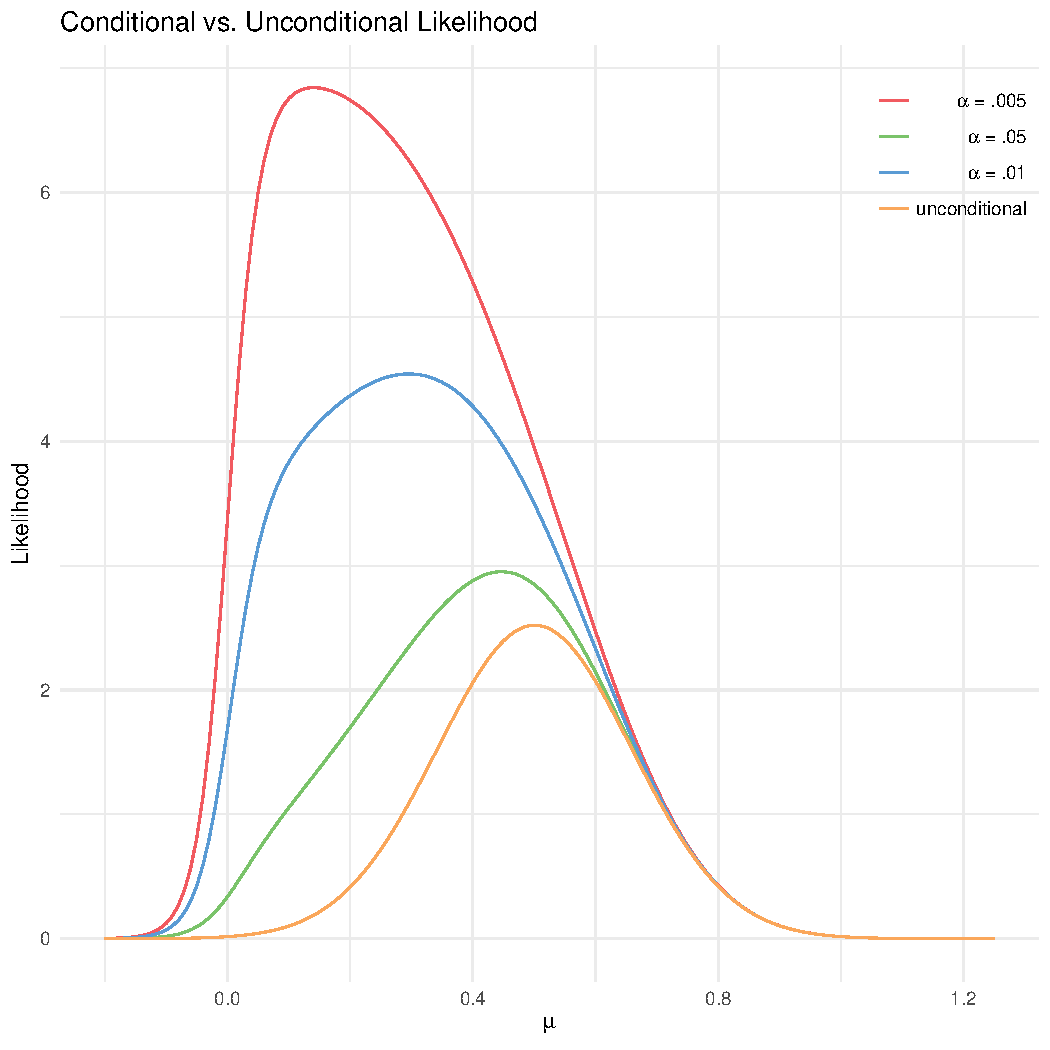
\includegraphics[width=4in]{figure/unnamed-chunk-5-1} 

}



\end{knitrout}
\end{figure}

In this case, the discovery data will have an effect on the amount of zero-valued global effects sampled because it skews the distribution to the right. However, since in this specific model we do not use the effect estimates from the discovery data, we essentially throw away any information regarding the size of the effect. These can be added in future models to better utilize the discovery data.


\subsection{Prior Specifications}


The choice of Cauchy priors for $\mu$ and $\sigma^2_{\beta}$ is based on simulation results. Both priors had mean zero and variance 1, based on the usual range of effect sizes in GWAS. The hyperparameters for $\xi$ were set to $a = b= \frac{1}{2}$. This distribution has a U-shape so that it favors extreme probabilities (0 or 1) more heavily than the values between them.  The normal approximation for the conditional likelihood model was chosen for its simplicity and because of the large sample sizes of GWAS, which allow for CLT assumptions.

For the Bayes Factor model, $a = b= \frac{9}{10}$. This is because for small p-values, the transformation of $\xi$ can be very extreme. For a GWAS p-value $p = 10^{-7}$ and $\xi \sim \textsf{Beta}(.5,.5)$ , $P( \xi' \leq 0.5) =$  $\ensuremath{4.74\times 10^{-11}}$ . For the flatter prior: $\xi \sim \textsf{Beta}(.9,.9)$, $P( \xi' \leq 0.5) =$ $\ensuremath{1.24\times 10^{-6}}$. The Bayes Factor model is extremely sensitive to the choice of prior as well as to the p-value. While the skew is appropriate for this particular prior, it would not necessarily make sense with a flat or informative prior.

\subsection{Methods}

Models were fit using R2jags and in the simpler cases, with original Metropolis Hastings algorithms. To specify distributions that are not part of the R2jags library, such as the conditional likelihood, we use the "ones trick", which is implement by creating artificial observations of a Bernoulli variable. Consider a prior for $\theta$ that is proportional to $\pi(\theta)$. If we set that Bernoulli variable "ones" is equal to 1 with probability $\pi(\theta)$, create an observation "ones"$= 1$, and set a uniform prior for $\theta$, then we are effectively creating a "posterior" for theta that is proportional to  $\pi(\theta)$ as intended. JAGS model functions for the hierarchical simulations can be found in the supplement.

All computed credible intervals are HPD (highest posterior density) intervals. A 95\% HPD interval is the 95\% of the sampled values with the highest density. HPD intervals are guaranteed to be the shortest intervals for that scale (they are not scale-invariant), and can give more reasonable answers for multimodal distributions than quantile-based intervals because they can be disjoint. Point estimates were calculated used the posterior median, so that these estimates would be invariant to transformations (e.g. log).

\section{Normal Simulation}\label{sec:normal}

This simulation study addresses on the first goal outlined in the introduction: if the data from one site is found to be significant, how can we report this discovery in a way that takes into account the winner's curse? 

\subsection{Data Generation}

To test the hypothesis $H_0: \mu = 0$ versus  $H_1: \mu \neq 0$, a fixed proportion (set at 0.5) of null vs. alternative hypotheses are generated. For each hypothesis $H_i$, let $\mu_i = 0$ in the null scenario and $\mu_i \sim \textsf{N}(0,1)$ in the alternative. The data $Y_i$ is generated from a normal distribution with mean $\mu_i$ and known variance 1, with sample size 100. If $Y_i$ is not significant at $\alpha = .05$, it is sampled again from the same distribution until the sufficient statistic is significant. This is done in order to properly compare the Bayesian approach with the conditional likelihood, which requires the data to be significant. The Bayes factor model as it is specified cannot be used in this scenario, since it only uses the p-value from the discovery site(s).

\subsection{Conditional Likelihood}

The credible intervals were estimated by treating the conditional likelihood as if it were a posterior distribution with an improper prior $p(\mu) = 1$, and obtaining the HPD region covering 95\%. Sampling was done through a Metropolis-Hastings algorithm.

\subsection{Posterior Distribution}




In the Bayesian case, the prior was set to the mixture model $p(\mu|\xi) = (1-\xi ) \delta_0(\mu)+ \xi\phi(\mu)$. In this case, $\xi = 0.5$ is a constant. Note that this is also the true data generating model. 

The marginal posterior distribution is 
\begin{equation}
P(\mu | Y ) = P(H_0|Y)P(\mu|Y, H_0) + P(H_1|Y)P(\mu|Y, H_1)
\end{equation}

The separate posteriors for $\mu$ are:
\begin{gather}
P(\mu|Y, H_0) = \delta_0(\mu)\\
P(\mu|Y, H_1) \sim \textsf{N}(\frac{n}{n+1}\bar Y, \frac{1}{n+1})
\end{gather}

The posterior for the alternative hypothesis can be calculated using its Bayes factor, BF and the prior odds, $\pi = \frac{(1-\xi)}{\xi}$: 
\begin{equation}
P(H_1| Y ) = \frac{\pi BF}{1+\pi BF}
\end{equation}

For this example, the prior odds are 1 (because the probability of $H_1 = \xi = 0.5$). The Bayes factor is
\begin{equation}
BF = \frac{L(\bar Y | H_1)}{L(\bar Y | H_0)} = \sqrt{n+1}* e^{\frac{n^2}{2(n+1)}(\bar Y)^2}
\end{equation}

This result comes from the fact that the marginal likelihood $L(\bar Y | H_1) \sim \textsf{N}(0, \frac{n}{n+1})$.


Putting these pieces together results in the marginal posterior for $\mu$, which can be used to generate samples to calculate credible intervals. 



\subsection{Results}


\subsubsection{Estimators}

\begin{knitrout}
\definecolor{shadecolor}{rgb}{0.969, 0.969, 0.969}\color{fgcolor}\begin{table}

\caption{\label{tab:unnamed-chunk-8}RMSE of 100 simulations}
\centering
\begin{tabular}[t]{r|r|r|r|r|r}
\hline
Bayes.mean & Bayes.median & Bayes.mode & cond.mean & cond.mode & naive\\
\hline
3.619 & 4.033 & 4.033 & 3.772 & 3.659 & 4.971\\
\hline
\end{tabular}
\end{table}


\end{knitrout}


\begin{figure}
\begin{knitrout}
\definecolor{shadecolor}{rgb}{0.969, 0.969, 0.969}\color{fgcolor}

{\centering 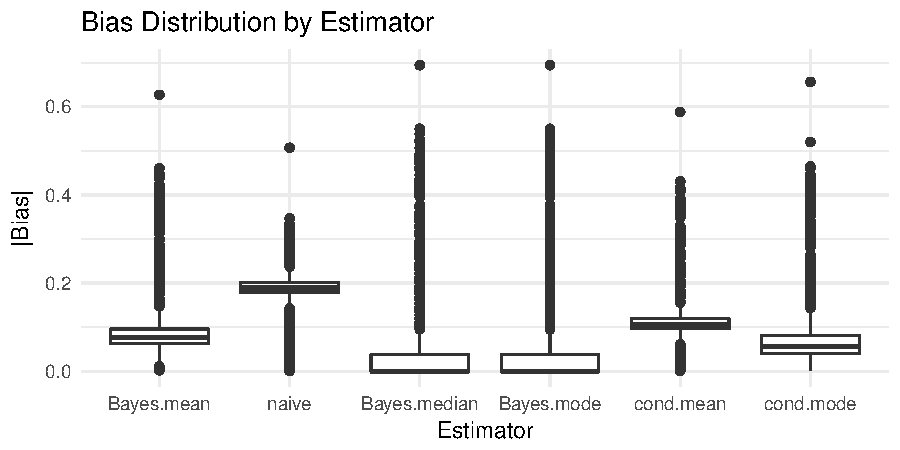
\includegraphics[width=4in]{figure/unnamed-chunk-9-1} 

}



\end{knitrout}
\end{figure}

The conditional likelihood mode (i.e. MLE) has the smallest bias (absolute error) for $\mu$ out of the frequentist estimators, while the Bayesian median and mode (which end up being the same) the smallest bias in the Bayesian framework. The RMSE for the Bayesian estimator (mean of the posterior) is the lowest, followed by the conditional mean and mode.

\subsubsection{Credible Intervals}




\begin{figure}
\begin{knitrout}
\definecolor{shadecolor}{rgb}{0.969, 0.969, 0.969}\color{fgcolor}

{\centering 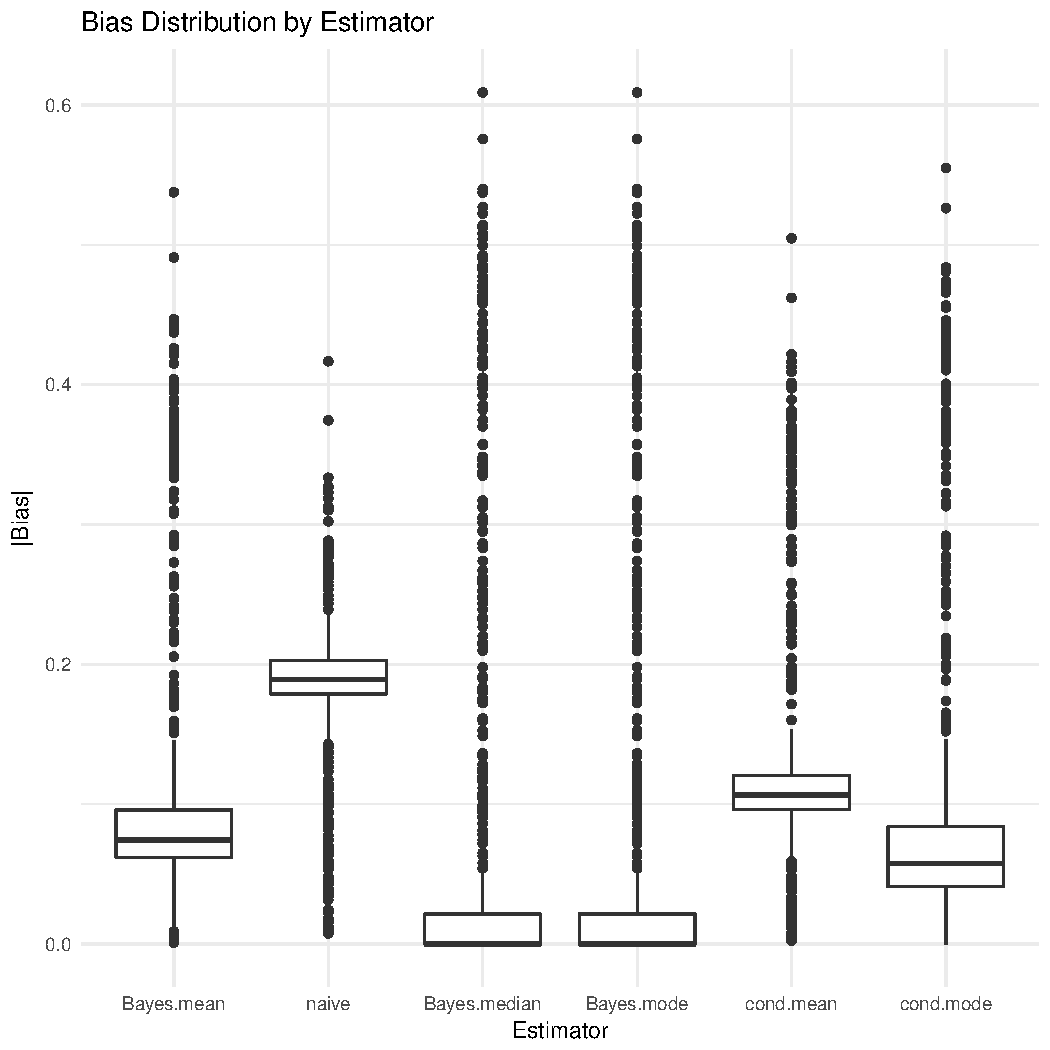
\includegraphics[width=4in]{figure/unnamed-chunk-11-1} 

}



\end{knitrout}
\end{figure}

The lines mark the $y = x$ line, and the length of naive confidence intervals (which are constant for fixed number of samples) on the x and y axes. The largest values for the significant statistic also correspond to the largest intervals in both cases. Note that the conditional likelihood credible intervals are almost always larger than the fully Bayesian credible intervals, but still mostly smaller than the naive ones. 

\subsubsection{Coverage}


The marginal coverage of the conditional likelihood credible interval C is 
\begin{equation}
P(\mu \in C|Y) = P(\mu \in C|H_0) P(H_0|Y)+P(\mu \in C|H_1) P(H_1|Y)
\end{equation}

This will be significantly higher than .95 for the cases in which $0 \in C$, since $P(\mu \in C|H_1) =0.95$ by definition, and  $P(\mu \in C|H_0) = I_{0 \in C}$. In this experiment, the expected coverage is $0.98$ for intervals with 0, and only $0.38$ for those that do not contain 0.  However, conditioning on the alternative hypothesis does not lead to an empirical coverage of 95\%. We can see that both methods are still significantly better than the naive one.



\subsubsection{Hypothesis Testing}


Due to the nature of p-values, an $\alpha = 0.05$ corresponds to a marginal posterior probability $P(H_1 | Y )$ of only $0.4$ for $N = 100$. This means that the 95\% credible interval for $\mu| Y$ will contain 0 every time. In terms of hypothesis testing, if we consider the strategy of rejecting the null when the interval does not contain 0, this level for $\alpha$ leads to no rejections.

\begin{knitrout}
\definecolor{shadecolor}{rgb}{0.969, 0.969, 0.969}\color{fgcolor}\begin{table}

\caption{\label{tab:unnamed-chunk-13}Naive method}
\centering
\begin{tabular}[t]{l|r|r}
\hline
  & Do not reject null & Reject null\\
\hline
0 & 0.274 & 0.443\\
\hline
1 & 0.127 & 0.156\\
\hline
\end{tabular}
\end{table}


\end{knitrout}

\begin{knitrout}
\definecolor{shadecolor}{rgb}{0.969, 0.969, 0.969}\color{fgcolor}\begin{table}

\caption{\label{tab:unnamed-chunk-14}Conditional Likelihood Method}
\centering
\begin{tabular}[t]{l|r}
\hline
  & Do not reject null\\
\hline
0 & 0.717\\
\hline
1 & 0.283\\
\hline
\end{tabular}
\end{table}


\end{knitrout}

\begin{knitrout}
\definecolor{shadecolor}{rgb}{0.969, 0.969, 0.969}\color{fgcolor}\begin{table}

\caption{\label{tab:unnamed-chunk-15}Bayesian Mixture Model}
\centering
\begin{tabular}[t]{l|r}
\hline
  & Do not reject null\\
\hline
0 & 0.717\\
\hline
1 & 0.283\\
\hline
\end{tabular}
\end{table}


\end{knitrout}

Despite never rejecting the null, the conditional likelihood and the Bayesian methods both perform better than the naive one in terms of "predicting" accurately. The naive method is especially problematic in that it has a higher Type 1 error (false positives) than true positives OR true negatives in the region of the data.

\section{Hierarchical Simulations}\label{sec:hierarchical}





This simulation study aims to deal with the second goal specified in the introduction. After an effect has been discovered, how can data from replication studies be combined with the original? In this scenario, we must account for the heterogeneity between sites; neglecting the uncertainty that comes from replication studies would lead to erroneously confident estimates of significance and effect size.



\subsection{Data Generation}

The data are generated from a hierarchical (i.e. mixed effect) logistic model as discribed in the models section: if truly associated, $\mu$ and $\sigma^2$ have (fixed) nonzero values;$\beta_j \sim \textsf{N}(\mu, \sigma^2)$. Otherwise, $\mu=\beta_j = 0,  \forall j$. 

To try to keep this simulation as close to the real data as possible, a preliminary logistic regression with random slope and random p53 coefficient by site was run. This led to the values of $\mu =0.203, \sigma^2 = 0.003$. The value of $\mu$ remained fixed through all the simulations, but different values of $\sigma$ were used to test the sensitivity of the models: $\sigma$, $\sigma/2$, $2\sigma$, and  $4\sigma$. The number of sites was set to 7, since results using 30 sites were almost identical. Each site had 1000 observations. A total of 100 simulated datasets was created each time.


100 datasets were also simulated under the null hypothesis. They were fit with the models described previously. 

\subsubsection{Finding "Discovery" Sites}

In this simulation study, a logistic regression with fixed effects for sites was conducted to find the site with the smallest p-value less than $\alpha$. If no sites matched this description, the data was resampled until at least one site was viable. The maximum likelihood estimate of this effect and its variance were added as data for the conditional likelihood model, and the p-value was added to the bayes factor approximation model.  The observations for this site were then taken out of the data.

\subsection{Results}











\subsubsection{RMSE of $\mu$}

As expected, the models performed more poorly as $\sigma$ increased. Out of the three proposed models (compared with the original), the fully bayesian and BF approximation models performed best when there was no true effect (since they were the only ones that that had this option). However, there were some simulated datasets where the bayes factor model estimate was actually nonzero and quite large, which suggests that it is not nearly as reliable as the bayesian model.


At small variances (s/2, s,  2s), the original and bayesian models outperform the others. This is not surprising since the other models only have access to $\frac{6}{7}$ of the data. The Bayesian model actually has a slightly higher lower RMSE than the other models when there is a true association.




\begin{knitrout}
\definecolor{shadecolor}{rgb}{0.969, 0.969, 0.969}\color{fgcolor}\begin{table}

\caption{\label{tab:unnamed-chunk-20}RMSE of $\mu$}
\centering
\begin{tabular}[t]{l|r|r|r|r|r}
\hline
  & mu=0 & s/2 & s & 2s & 4s\\
\hline
Bayesian & 0.000 & 0.025 & 0.037 & 0.053 & 0.099\\
\hline
Cond Likelihood & 0.018 & 0.027 & 0.034 & 0.055 & 0.098\\
\hline
BF Approx & 0.012 & 0.024 & 0.031 & 0.053 & 0.097\\
\hline
Original & 0.024 & 0.025 & 0.031 & 0.052 & 0.099\\
\hline
\end{tabular}
\end{table}


\end{knitrout}


\begin{figure}
\begin{knitrout}
\definecolor{shadecolor}{rgb}{0.969, 0.969, 0.969}\color{fgcolor}

{\centering 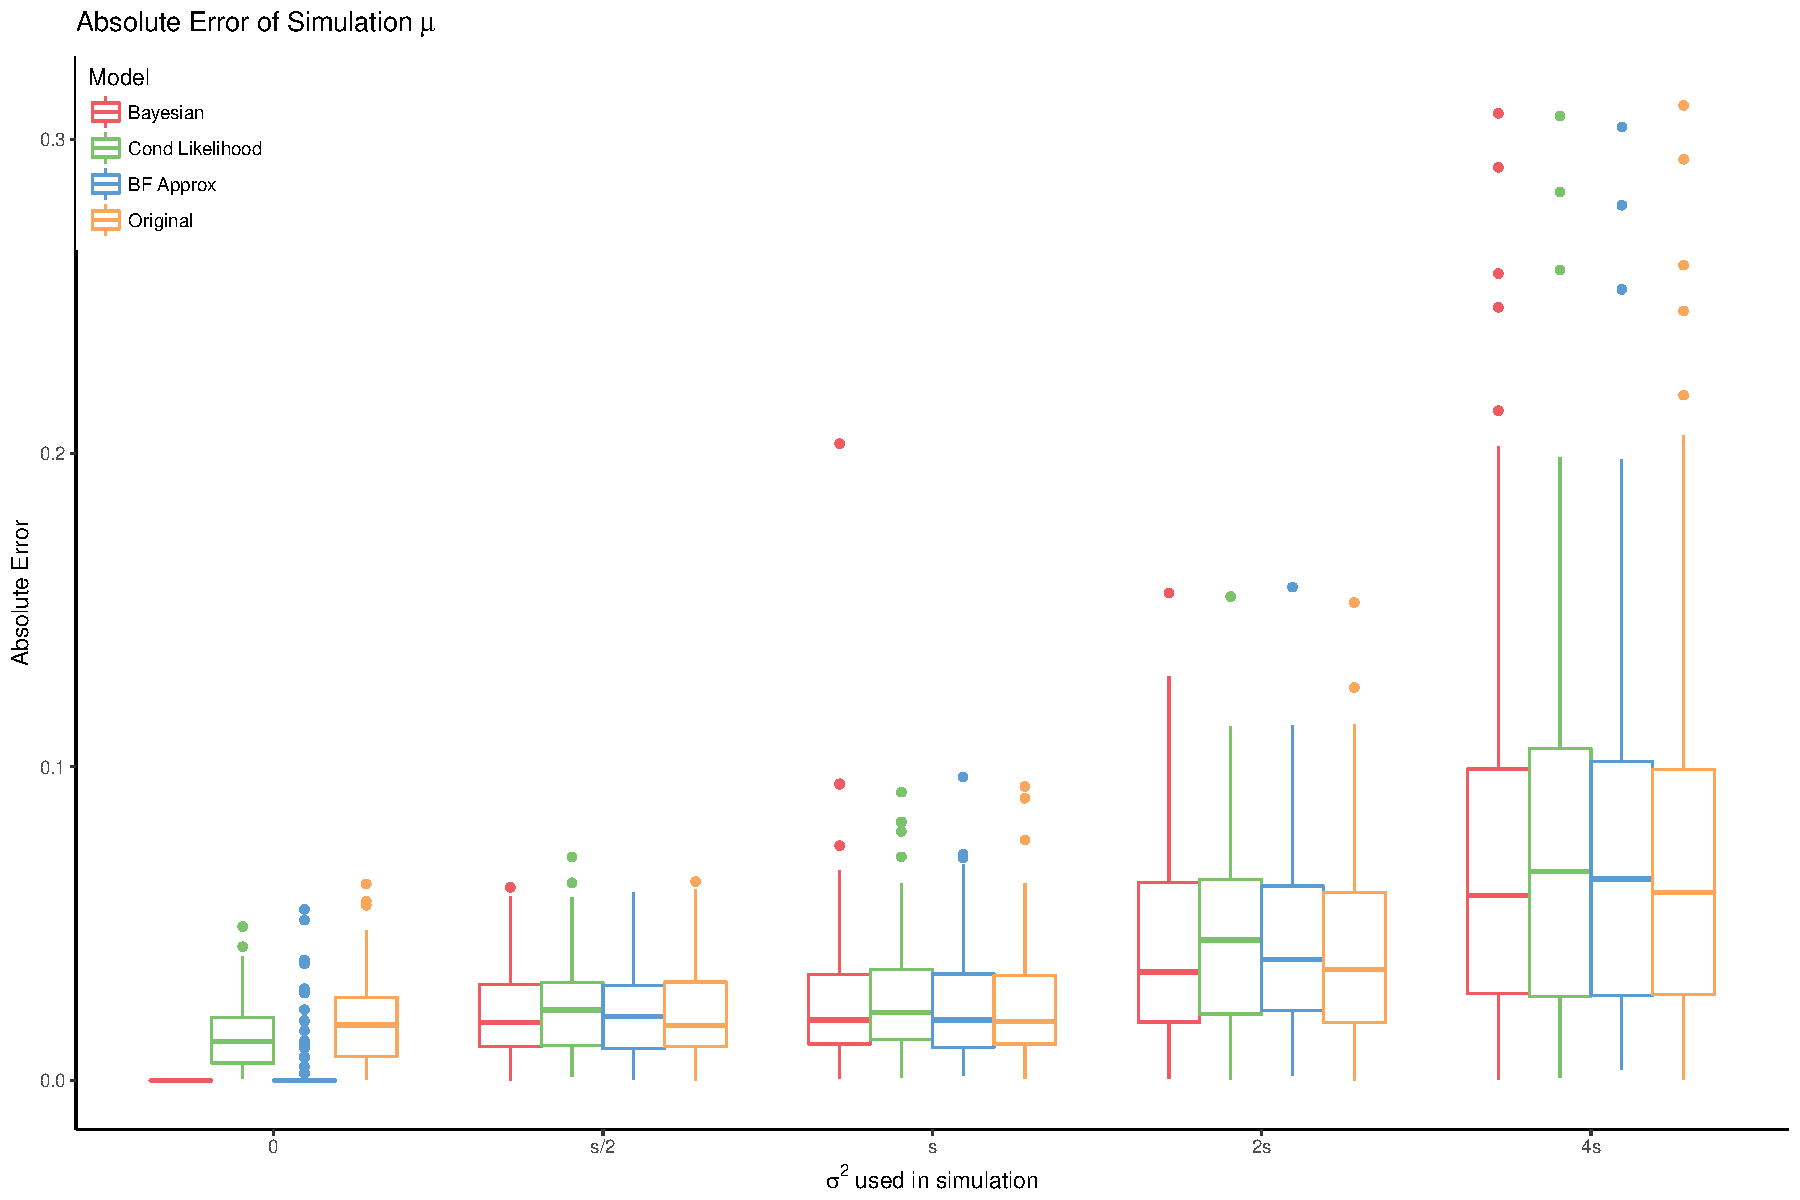
\includegraphics[width=4in]{figure/unnamed-chunk-21-1} 

}



\end{knitrout}
\end{figure}

\subsubsection{Coverage of $\mu$}

The conditional likelihood and BF approximation models are the most conservative, with the intervals covering 0 more times than the  others for large values of $\sigma$. All models have very high coverage in general.

The Bayesian model had the shortest intervals, and the original model had the largest. Thus, even though the coverage and RMSE are around the same, the new models are preferable to the original. This does not apply to the simulation with $\sigma=4s$, because $4s>\mu$, which leads to more negative site effects. Thus, it makes sense for models to have wider credible intervals for these simulations. 


\begin{knitrout}
\definecolor{shadecolor}{rgb}{0.969, 0.969, 0.969}\color{fgcolor}\begin{table}

\caption{\label{tab:unnamed-chunk-22}Proportion of Credible Intervals containing $\mu$}
\centering
\begin{tabular}[t]{l|r|r|r|r|r}
\hline
  & mu=0 & s/2 & s & 2s & 4s\\
\hline
Bayesian & 1.00 & 1 & 0.98 & 0.98 & 0.97\\
\hline
Cond Likelihood & 0.71 & 1 & 0.95 & 0.95 & 0.96\\
\hline
BF Approx & 0.98 & 1 & 0.97 & 0.98 & 0.97\\
\hline
Original & 0.96 & 1 & 1.00 & 0.99 & 0.95\\
\hline
\end{tabular}
\end{table}


\end{knitrout}

\begin{knitrout}
\definecolor{shadecolor}{rgb}{0.969, 0.969, 0.969}\color{fgcolor}\begin{table}

\caption{\label{tab:unnamed-chunk-23}Proportion of Credible Intervals containing 0}
\centering
\begin{tabular}[t]{l|r|r|r|r|r}
\hline
  & mu=0 & s/2 & s & 2s & 4s\\
\hline
Bayesian & 1.00 & 0.02 & 0.08 & 0.13 & 0.50\\
\hline
Cond Likelihood & 0.71 & 0.00 & 0.01 & 0.11 & 0.51\\
\hline
BF Approx & 0.98 & 0.00 & 0.00 & 0.11 & 0.51\\
\hline
Original & 0.96 & 0.00 & 0.01 & 0.14 & 0.42\\
\hline
\end{tabular}
\end{table}


\end{knitrout}


\begin{figure}
\begin{knitrout}
\definecolor{shadecolor}{rgb}{0.969, 0.969, 0.969}\color{fgcolor}

{\centering 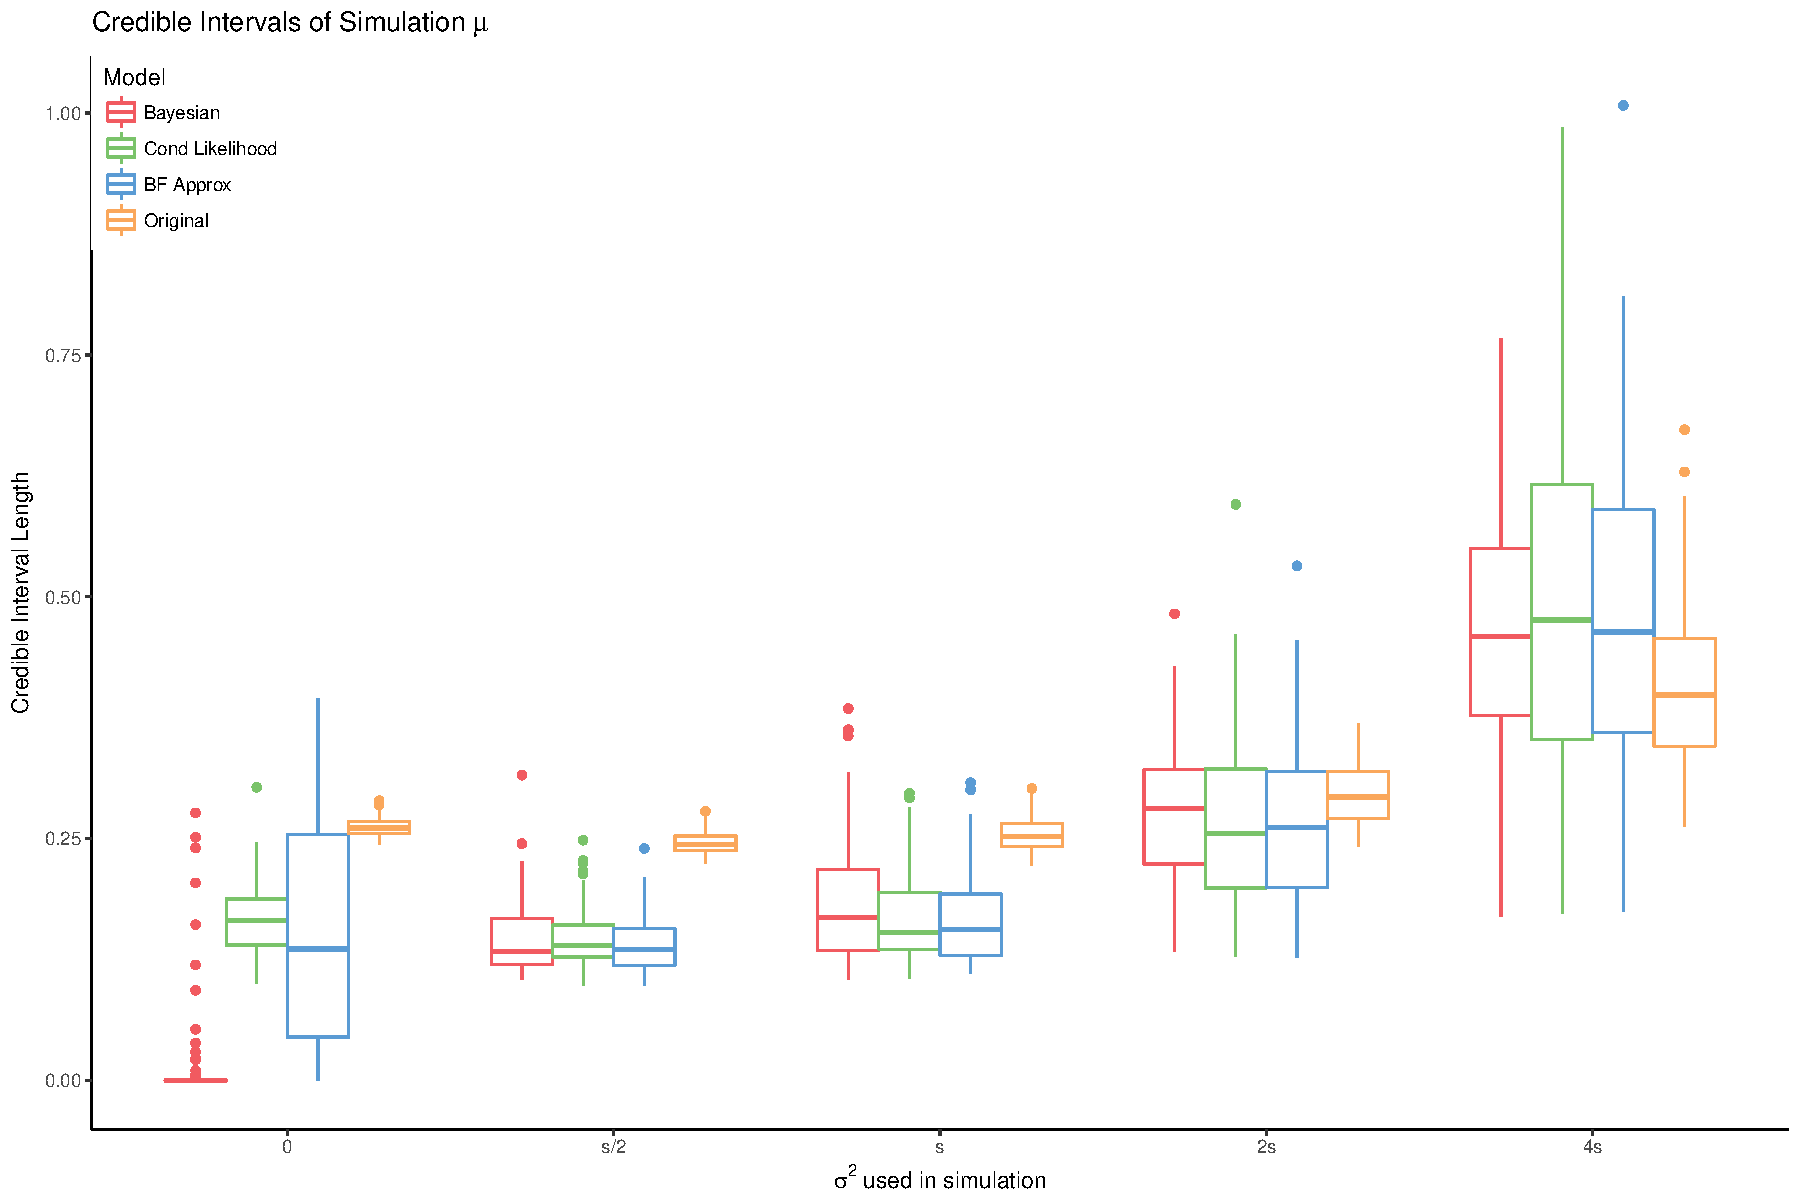
\includegraphics[width=4in]{figure/unnamed-chunk-24-1} 

}



\end{knitrout}
\end{figure}

\subsubsection{Probability of Association $\xi$}

While one would expect the probability of being associated ($\xi$) to also increase with $\sigma$, this was not true for either the fully bayesian model nor the bayes factor approximation one, both of which had consistent posterior estimates of $\xi$. Similarly, the proportion of nonzero $\mu$ samples from the posterior (this is the same as the proportion of times the latent variable $i = 1$), was almost 1 for the truly associated cases, and close to zero for true null. One thing to consider is that under the null hypothesis, the variance across sites would actually be zero, which is why the models identified the association so decisively.

For the simulations that had no true effect, the Bayes Factor approximation model has much larger median $\xi$ and greater proportion of sampled $H_1$ because the mass of the distribution of $\xi$ is shifted towards 1 by the Bayes Factor transformation. Thus, even though the proportion of $H_1$ is quite low (and the median of $\mu$ is 0), the mean of $\xi$ is greater than $0.5$.


\begin{knitrout}
\definecolor{shadecolor}{rgb}{0.969, 0.969, 0.969}\color{fgcolor}\begin{table}

\caption{\label{tab:unnamed-chunk-25}Average of Posterior Median $\xi$}
\centering
\begin{tabular}[t]{l|r|r|r|r|r}
\hline
  & mu=0 & s/2 & s & 2s & 4s\\
\hline
Bayesian & 0.210 & 0.836 & 0.830 & 0.832 & 0.837\\
\hline
BF Approx & 0.847 & 0.991 & 0.992 & 0.994 & 0.998\\
\hline
\end{tabular}
\end{table}


\end{knitrout}

\begin{knitrout}
\definecolor{shadecolor}{rgb}{0.969, 0.969, 0.969}\color{fgcolor}\begin{table}

\caption{\label{tab:unnamed-chunk-26}Average Proportion of $H_1$}
\centering
\begin{tabular}[t]{l|r|r|r|r|r}
\hline
  & mu=0 & s/2 & s & 2s & 4s\\
\hline
Bayesian & 0.132 & 0.998 & 0.989 & 0.989 & 0.996\\
\hline
BF Approx & 0.501 & 1.000 & 1.000 & 1.000 & 1.000\\
\hline
\end{tabular}
\end{table}


\end{knitrout}


\subsubsection{Sensitivity of Conditional Likelihood Method to Changes in $\alpha$}

The conditional likelihood method with random effects is robust to changes in the level $\alpha$. To test this, we consider 5 different levels: $0.05, 0.01, 0.005, 0.001, 10^{-7}$. 100 datasets were sampled, for which at least one location was significant at the smallest $\alpha$ level. The conditional likelihood model with random effects and without was then fitted for each level. 



\begin{knitrout}
\definecolor{shadecolor}{rgb}{0.969, 0.969, 0.969}\color{fgcolor}\begin{table}

\caption{\label{tab:unnamed-chunk-28}RMSE of $\mu$}
\centering
\begin{tabular}[t]{l|r|r|r}
\hline
  & 0 & s & 4s\\
\hline
0.05 & 0.019 & 0.039 & 0.101\\
\hline
0.01 & 0.020 & 0.040 & 0.090\\
\hline
0.005 & 0.019 & 0.040 & 0.099\\
\hline
0.001 & 0.019 & 0.038 & 0.098\\
\hline
1e-07 & NA & 0.039 & 0.097\\
\hline
\end{tabular}
\end{table}


\end{knitrout}



\begin{figure}
\begin{knitrout}
\definecolor{shadecolor}{rgb}{0.969, 0.969, 0.969}\color{fgcolor}

{\centering 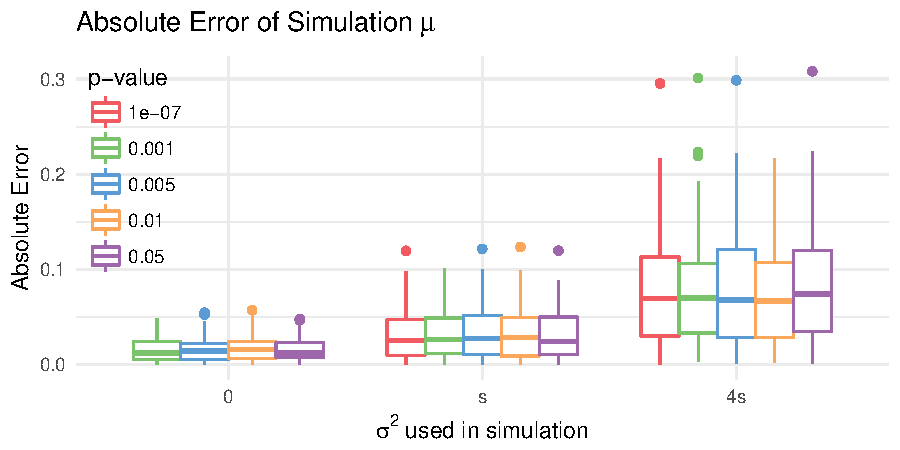
\includegraphics[width=4in]{figure/unnamed-chunk-29-1} 

}



\end{knitrout}
\end{figure}


\begin{figure}
\begin{knitrout}
\definecolor{shadecolor}{rgb}{0.969, 0.969, 0.969}\color{fgcolor}

{\centering 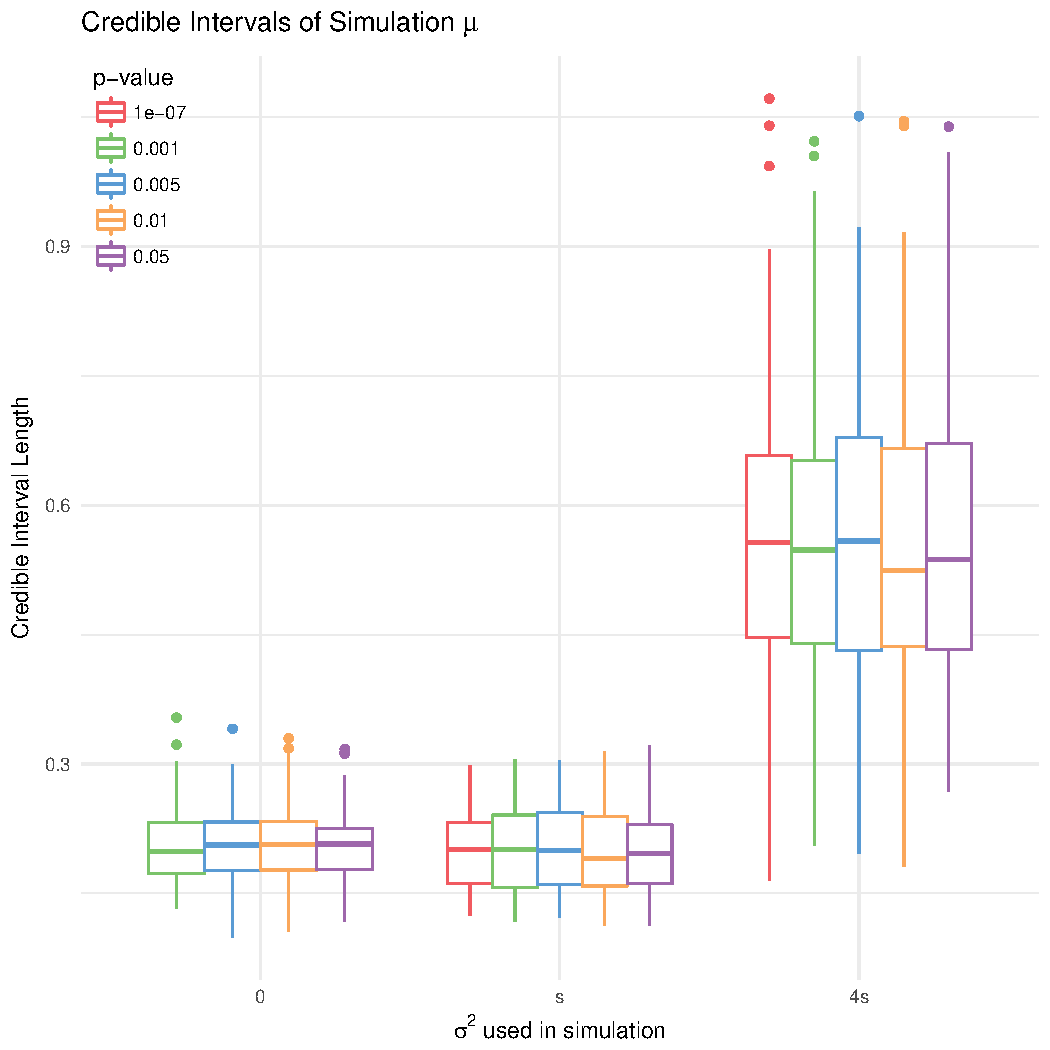
\includegraphics[width=4in]{figure/unnamed-chunk-30-1} 

}



\end{knitrout}
\end{figure}
This model shows little difference across levels of $\alpha$.

\section{Analysis of TP53}\label{sec:tp53}
---------------
\subsection{Models}


Each model adjusts for study site, reference age, and personal history of breast cancer. History of breast cancer is treated as a fixed effect, and the rest of the covariates's coefficients are treated as normally distributed random effects. 

\begin{gather}
P(Y_{ij}=1| \beta^{site}_{ j}, \beta^{p53}_{j}, \beta^{age}_{j},\beta^{BC}) = \textsf{logit}^{-1}(\beta^{site}_{ j}+ \beta^{p53}_{j}*p53_{ij}+ \beta^{age}_{j}*age_{ij}+\beta^{BC}* BC_{ij})\\
\beta^{site}_{ j}|\mu_{site}, \sigma_{site}^{2}\sim \textsf{N}(\mu_{site}, \sigma_{site}^{2})\\
\beta^{age}_{j}|\mu_{age}, \sigma^{2}_{age}\sim \textsf{N}(\mu_{age}, \sigma^{2}_{age})\\
\beta^{\text{BC}}, \mu_{age},\mu_{site}\sim \textsf{N}(0,0.1)\\
\sigma_{age},\sigma_{site} \sim \textsf{invGamma}(1, 0.05)
\end{gather}

The p53 variable's site-specific log OR priors were defined using the models described previously. The fully Bayesian model was fit jointly as well as marginally. Since the results were very similar, the marginal models were used for computational efficiency and clarity of interpretation. Results from the joint analysis can be found in the supplement.

\subsection{Results}







\begin{knitrout}
\definecolor{shadecolor}{rgb}{0.969, 0.969, 0.969}\color{fgcolor}

{\centering 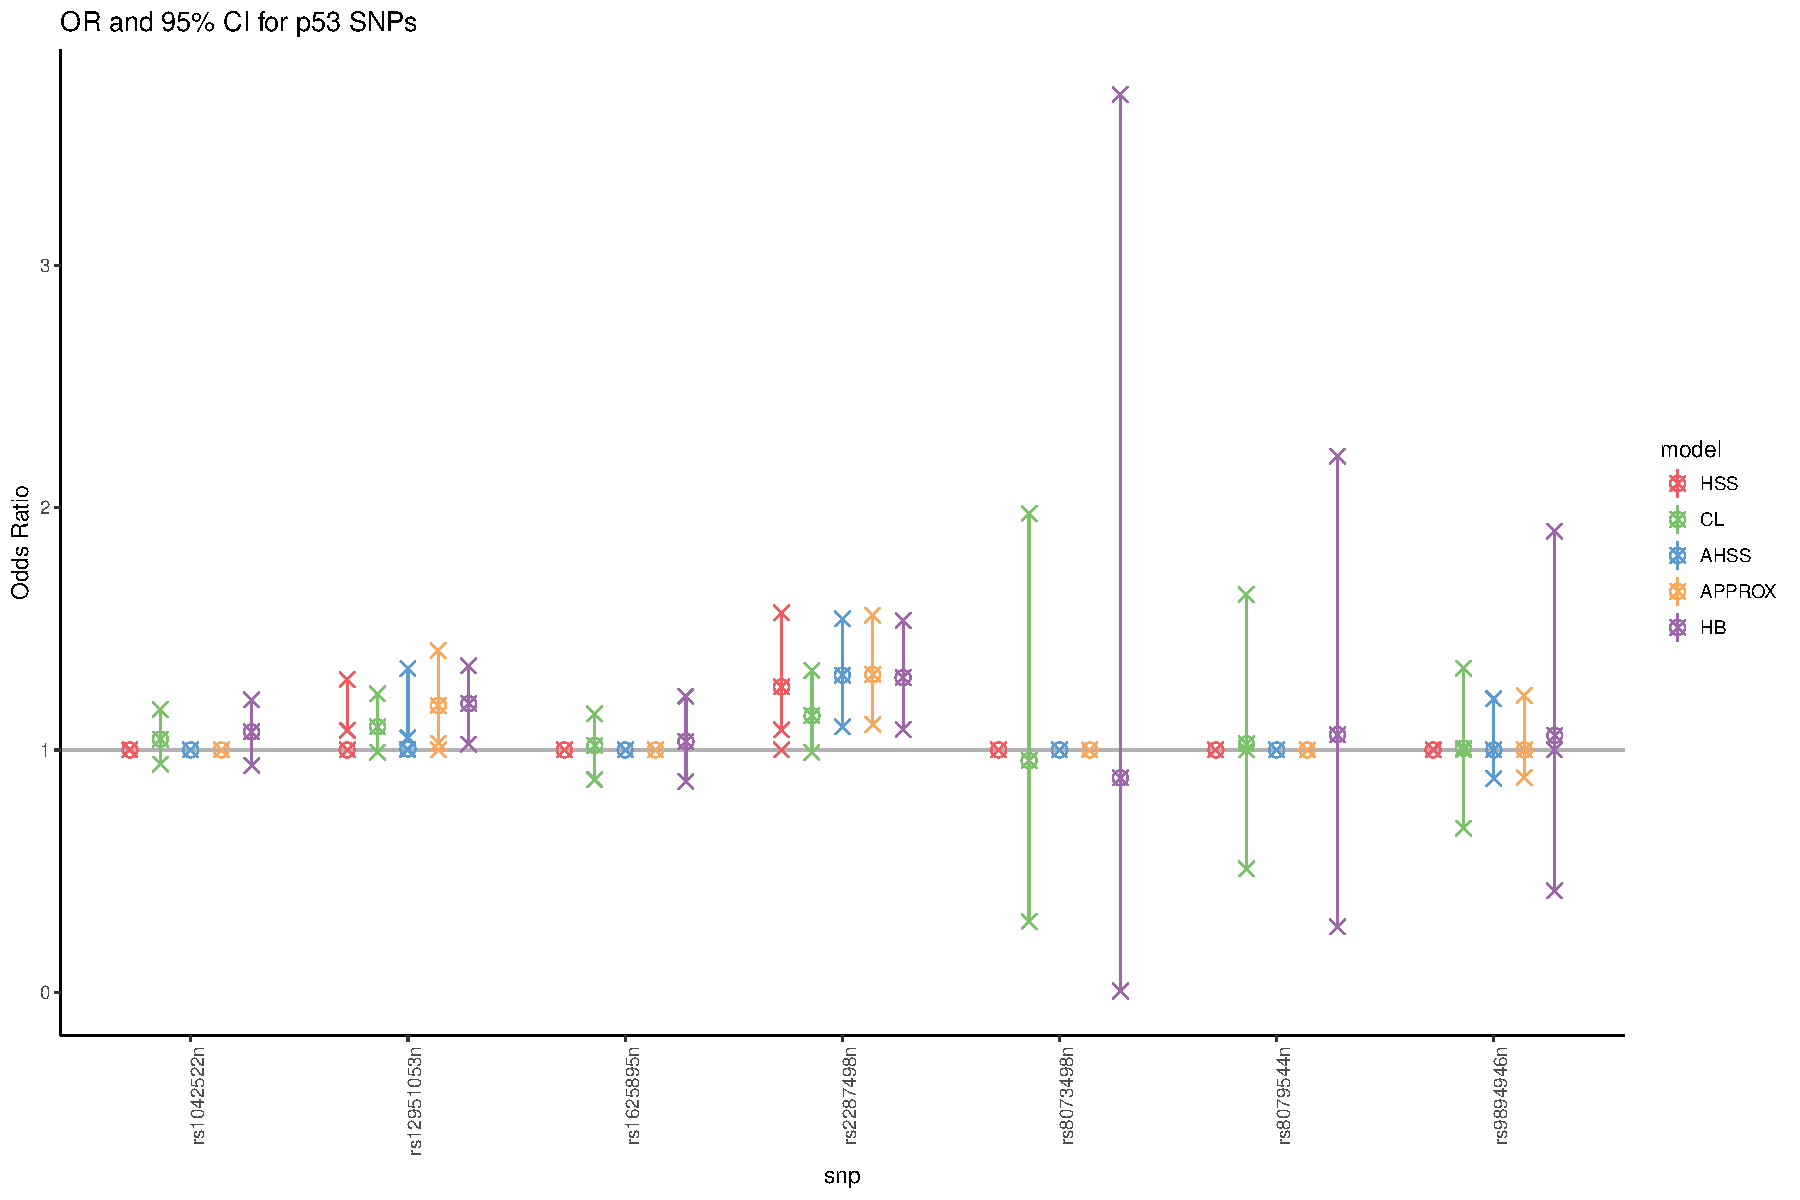
\includegraphics[width=4in]{figure/unnamed-chunk-32-1} 

}



\end{knitrout}

The new models shrunk estimates towards 0 for all SNPs. The BF approximation model set all point estimates to zero, as did the fully Bayesian model with the exception of one. This is the same SNP (rs2287498n) 
that was detected as significant in the MISA analysis \cite{schildkraut2010association}. However, the fully Bayesian credible interval for this SNP is longer than the original model's, indicating that if data closer to 0 were collected and added to the analysis, the interval would become disjoint with the point mass at zero and a narrower nozero interval.  The Bayes factor model credible interval for this SNP is the same as the original credible interval. This is because the p-value was small enough to skew the distribution towards one, and there was enough information in the validation data that the chain got "stuck" at $H = 1$. Although the conditional likelihood model does not set any estimates to zero, all its credible intervals contain zero. These results are consistent with those from recent GWAS \cite{phelan2017identification}, which found no association between any of the TP53 SNPs and cancer.

Below are the full tables of OR by site and SNP.

\begin{table}

\caption{\label{tab:unnamed-chunk-33}rs9894946n}
\centering
\resizebox{\linewidth}{!}{\begin{tabular}[t]{l|l|l|l|l|l|l|l|l}
\hline
  & original estimate & original CI & bayesian estimate & bayesian CI & CL estimate & CL CI & BF estimate & BF CI\\
\hline
AUS & 0.969 & 0.737 - 1.245 & 1 & 1 - 1 & 0.985 & 0.769 - 1.197 & 1 & 0.886 - 1.097\\
\hline
HAW & 0.943 & 0.405 - 1 ,  1 - 1.485 & 1 & 1 - 1 & 0.987 & 0.565 - 1.35 & 1 & 0.753 - 1.181\\
\hline
MAY & 0.962 & 0.714 - 1.258 & 1 & 1 - 1 & 0.978 & 0.746 - 1.2 & 1 & 0.869 - 1.101\\
\hline
POL & 1.486 & 0.965 - 2.198 & 1 & 1 - 1 & 1.079 & 0.878 - 1 ,  1 - 1.461 & 1 & 0.93 - 1.128 ,  1.204 - 1.621\\
\hline
Overall & 1.058 & 0.385 - 1.82 & 1 & 1 - 1 & 1.008 & 0.691 - 1.396 & 1 & 0.862 - 1.249\\
\hline
\end{tabular}}
\end{table}
\begin{table}

\caption{\label{tab:unnamed-chunk-33}rs12951053n}
\centering
\resizebox{\linewidth}{!}{\begin{tabular}[t]{l|l|l|l|l|l|l|l|l}
\hline
  & original estimate & original CI & bayesian estimate & bayesian CI & CL estimate & CL CI & BF estimate & BF CI\\
\hline
AUS & 1.239 & 1.029 - 1.513 & 1 & 0.97 - 1.065 ,  1.067 - 1.386 & 1.139 & 0.975 - 1 ,  1.001 - 1.405 & 1 & 0.983 - 1.375\\
\hline
HAW & 1.185 & 0.842 - 1 ,  1 - 1.497 & 1 & 0.933 - 1.372 & 1.093 & 0.859 - 1.343 & 1 & 0.934 - 1.364\\
\hline
MAL & 1.19 & 0.931 - 1.445 & 1 & 0.953 - 1.348 & 1.108 & 0.929 - 1.339 & 1 & 0.959 - 1.335\\
\hline
MAY & 1.209 & 0.975 - 1.524 & 1 & 0.951 - 1.378 & 1.113 & 0.941 - 1 ,  1 - 1.338 & 1 & 0.954 - 1.343\\
\hline
NCO & 1.261 & 1.036 - 1.626 & 1 & 0.958 - 1.439 & 1.074 & 0.818 - 1 ,  1 - 1.295 & 1 & 0.893 - 1.357\\
\hline
NEC & 1.199 & 0.973 - 1.477 & 1 & 0.955 - 1.349 & 1.076 & 0.885 - 1.257 & 1 & 0.941 - 1.297\\
\hline
NHS & 1.148 & 0.742 - 1.407 & 1 & 0.897 - 1.35 & 1.099 & 0.888 - 1 ,  1 - 1.337 & 1 & 0.938 - 1.35\\
\hline
POL & 1.183 & 0.897 - 1.44 & 1 & 0.946 - 1.344 & 1.099 & 0.91 - 1.338 & 1 & 0.937 - 1.341\\
\hline
SEA & 1.136 & 0.844 - 1.35 & 1 & 0.93 - 1.301 & 1.117 & 0.929 - 1 ,  1 - 1.381 & 1 & 0.946 - 1.379\\
\hline
STA & 1.188 & 0.896 - 1 ,  1 - 1.471 & 1 & 0.94 - 1.365 & 1.117 & 0.944 - 1 ,  1 - 1.352 & 1 & 0.949 - 1.35\\
\hline
UCI & 1.18 & 0.89 - 1.45 & 1 & 0.948 - 1.352 & 1.08 & 0.931 - 1.24 & 1 & 0.942 - 1.367\\
\hline
UKO & 1.209 & 0.915 - 1.514 & 1 & 0.954 - 1.386 & 1.098 & 0.959 - 1.285 & 1 & 0.965 - 1.432\\
\hline
USC & 1.207 & 0.982 - 1.488 & 1 & 0.954 - 1.35 & 1.07 & 0.932 - 1.234 & 1 & 0.943 - 1.334\\
\hline
Overall & 1.19 & 1.023 - 1.36 & 1 & 0.988 - 1.32 & 1.1 & 0.989 - 1 ,  1 - 1.235 & 1 & 0.983 - 1.312\\
\hline
\end{tabular}}
\end{table}
\begin{table}

\caption{\label{tab:unnamed-chunk-33}rs1625895n}
\centering
\resizebox{\linewidth}{!}{\begin{tabular}[t]{l|l|l|l|l|l|l|l|l}
\hline
  & original estimate & original CI & bayesian estimate & bayesian CI & CL estimate & CL CI & BF estimate & BF CI\\
\hline
AUS & 1.005 & 0.803 - 1.216 & 1 & 1 - 1 & 1.006 & 0.826 - 1.166 & 1 & 1 - 1\\
\hline
HAW & 1.012 & 0.699 - 1.287 & 1 & 1 - 1 & 1.011 & 0.751 - 1 ,  1 - 1.23 & 1 & 1 - 1\\
\hline
MAL & 1.051 & 0.844 - 1.303 & 1 & 1 - 1 & 1.033 & 0.859 - 1 ,  1 - 1.234 & 1 & 1 - 1\\
\hline
MAY & 1.043 & 0.843 - 1.295 & 1 & 1 - 1 & 1.031 & 0.856 - 1.229 & 1 & 1 - 1\\
\hline
NCO & 0.991 & 0.789 - 1 ,  1 - 1.184 & 1 & 1 - 1 & 1.001 & 0.818 - 1.158 & 1 & 1 - 1\\
\hline
POL & 1.099 & 0.856 - 1.535 & 1 & 1 - 1 & 1.033 & 0.863 - 1 ,  1 - 1.238 & 1 & 1 - 1\\
\hline
SEA & 1.042 & 0.832 - 1.266 & 1 & 1 - 1 & 1.015 & 0.811 - 1.208 & 1 & 1 - 1\\
\hline
STA & 1.019 & 0.78 - 1 ,  1 - 1.268 & 1 & 1 - 1 & 1.037 & 0.912 - 1.222 & 1 & 1 - 1\\
\hline
Overall & 1.034 & 0.878 - 1.218 & 1 & 1 - 1 & 1.02 & 0.889 - 1.151 & 1 & 1 - 1\\
\hline
\end{tabular}}
\end{table}
\begin{table}

\caption{\label{tab:unnamed-chunk-33}rs1042522n}
\centering
\resizebox{\linewidth}{!}{\begin{tabular}[t]{l|l|l|l|l|l|l|l|l}
\hline
  & original estimate & original CI & bayesian estimate & bayesian CI & CL estimate & CL CI & BF estimate & BF CI\\
\hline
AUS & 1.047 & 0.85 - 1.217 & 1 & 1 - 1 & 1.032 & 0.857 - 1.179 & 1 & 1 - 1\\
\hline
HAW & 1.053 & 0.773 - 1 ,  1 - 1.272 & 1 & 1 - 1 & 1.038 & 0.833 - 1 ,  1 - 1.246 & 1 & 1 - 1\\
\hline
MAL & 1.086 & 0.934 - 1.26 & 1 & 1 - 1 & 1.062 & 0.935 - 1.218 & 1 & 1 - 1\\
\hline
MAY & 1.099 & 0.939 - 1.308 & 1 & 1 - 1 & 1.07 & 0.935 - 1.255 & 1 & 1 - 1\\
\hline
NCO & 1.067 & 0.899 - 1.244 & 1 & 1 - 1 & 1.048 & 0.897 - 1.206 & 1 & 1 - 1\\
\hline
POL & 1.117 & 0.927 - 1.409 & 1 & 1 - 1 & 1.045 & 0.905 - 1.199 & 1 & 1 - 1\\
\hline
SEA & 1.063 & 0.881 - 1.227 & 1 & 1 - 1 & 1.048 & 0.886 - 1.212 & 1 & 1 - 1\\
\hline
STA & 1.068 & 0.878 - 1.261 & 1 & 1 - 1 & 1.051 & 0.941 - 1.186 & 1 & 1 - 1\\
\hline
Overall & 1.073 & 0.938 - 1.216 & 1 & 1 - 1 & 1.048 & 0.936 - 1.163 & 1 & 1 - 1\\
\hline
\end{tabular}}
\end{table}
\begin{table}

\caption{\label{tab:unnamed-chunk-33}rs8079544n}
\centering
\resizebox{\linewidth}{!}{\begin{tabular}[t]{l|l|l|l|l|l|l|l|l}
\hline
  & original estimate & original CI & bayesian estimate & bayesian CI & CL estimate & CL CI & BF estimate & BF CI\\
\hline
MAY & 1.092 & 0.685 - 1.645 & 1 & 1 - 1 & 1.063 & 0.728 - 1.602 & 1 & 1 - 1\\
\hline
NCO & 1.093 & 0.779 - 1.481 & 1 & 1 - 1 & 0.991 & 0.583 - 1.376 & 1 & 1 - 1\\
\hline
POL & 0.986 & 0.516 - 1.422 & 1 & 1 - 1 & 1.025 & 0.875 - 1.227 & 1 & 1 - 1\\
\hline
Overall & 1.057 & 0.225 - 1 ,  1 - 1.896 & 1 & 1 - 1 & 1.027 & 0.484 - 1 ,  1 - 1.573 & 1 & 1 - 1\\
\hline
\end{tabular}}
\end{table}
\begin{table}

\caption{\label{tab:unnamed-chunk-33}rs2287498n}
\centering
\resizebox{\linewidth}{!}{\begin{tabular}[t]{l|l|l|l|l|l|l|l|l}
\hline
  & original estimate & original CI & bayesian estimate & bayesian CI & CL estimate & CL CI & BF estimate & BF CI\\
\hline
HAW & 1.284 & 0.887 - 1.734 & 1.287 & 0.806 - 1 ,  1.001 - 1.764 & 1.126 & 0.829 - 1.475 & 1.293 & 0.896 - 1.66\\
\hline
MAL & 1.259 & 0.991 - 1.531 & 1.271 & 0.931 - 0.999 ,  1.002 - 1.566 & 1.144 & 0.928 - 1.395 & 1.276 & 1.012 - 1.548\\
\hline
MAY & 1.347 & 1.057 - 1.844 & 1.346 & 0.984 - 0.998 ,  1.003 - 1.87 & 1.121 & 0.904 - 1.357 & 1.247 & 0.959 - 1.523\\
\hline
NCO & 1.353 & 1.073 - 1.717 & 1.353 & 1.049 - 1.771 & 1.141 & 0.889 - 1 ,  1 - 1.465 & 1.289 & 0.973 - 1.647\\
\hline
POL & 1.278 & 0.932 - 1.597 & 1.284 & 0.895 - 0.999 ,  1 - 1.69 & 1.137 & 0.902 - 1.448 & 1.291 & 0.96 - 0.999 ,  1.001 - 1.625\\
\hline
SEA & 1.226 & 0.909 - 1.477 & 1.236 & 0.873 - 1 ,  1 - 1.533 & 1.207 & 0.981 - 1.623 & 1.38 & 1.092 - 1.802\\
\hline
STA & 1.284 & 0.935 - 1.628 & 1.287 & 0.896 - 1 ,  1 - 1.717 & 1.123 & 0.951 - 1.38 & 1.362 & 1.061 - 1.777\\
\hline
UKO & 1.28 & 0.909 - 1.594 & 1.285 & 0.887 - 0.998 ,  1 - 1.667 & 1.124 & 0.966 - 1.364 & 1.358 & 1.088 - 1.691\\
\hline
USC & 1.375 & 1.102 - 1.846 & 1.375 & 1.053 - 1.924 & 1.097 & 0.923 - 1.298 & 1.289 & 0.972 - 1.612\\
\hline
Overall & 1.296 & 1.087 - 1.537 & 1.3 & 1.037 - 1.582 & 1.138 & 0.984 - 1.323 & 1.306 & 1.114 - 1.544\\
\hline
\end{tabular}}
\end{table}
\begin{table}

\caption{\label{tab:unnamed-chunk-33}rs8073498n}
\centering
\resizebox{\linewidth}{!}{\begin{tabular}[t]{l|l|l|l|l|l|l|l|l}
\hline
  & original estimate & original CI & bayesian estimate & bayesian CI & CL estimate & CL CI & BF estimate & BF CI\\
\hline
MAY & 0.921 & 0.724 - 1.144 & 1 & 1 - 1 & 0.952 & 0.762 - 1.158 & 1 & 0.989 - 1.003\\
\hline
NCO & 0.844 & 0.695 - 0.989 & 1 & 1 - 1 & 0.96 & 0.824 - 1.045 & 1 & 0.962 - 1.023\\
\hline
Overall & 0.876 & 0.003 - 3.61 & 1 & 1 - 1 & 0.952 & 0.263 - 1.786 & 1 & 0.979 - 1.016\\
\hline
\end{tabular}}
\end{table}


\section{Conclusion}\label{sec:conclusion}


We expand on three ideas from current literature to deal with the winner's curse by reducing the selection effect in initial studies that test for significance, as well as in replicated ones that aim to validate previous discoveries. The fully Bayesian model uses all the data to make inference and uses a binary latent variable to model the true association. This is equivalent to a spike and slab prior, or to model averaging with two possible models: the null and the alternative.  The conditional likelihood method uses the likelihood of the estimate conditional on being significant. This is a frequentist approach to selection bias, and it depends on the significance test level as well as the effect estimate and standard error. The conditional likelihood is then used as a prior in the (Bayesian) validation analysis. The Bayes factor approximation method uses an upper bound on the Bayes factor that is only dependent on the p-value to calculate a "best-case scenario" posterior probability of the alternative hypothesis. The distribution that arises from this transformation is used as the prior of the association probability in the validation analysis. This approach also has a frequentist component, since p-values are used, but is a step towards the Bayesian framework since the only function of the p-value is to approximate the Bayes Factor. All models improve upon naive methods in the discovery phase, as shown in the normal simulation study, as well as the validation phase, as shown in the hierarchical simulation study and analysis of p53 data.

One clear advantage of the fully Bayesian model is that it can perform testing and estimation simultaneously. This means all the data is used once, which is why the credible intervals are smaller and the RMSE is lower in the simulations. However, it is not always feasible to implement if the discovery data is unavailable. Furthermore, Bayesian methods are not enough to not guarantee bias correction. They must take into account the selection mechanism (as is done here), and also report the uncertainty that is associated with this. Ignoring the selection effect or reporting only the selected interval can lead to paradoxes, especially for conjugate priors in multivariate inference, as was the case with the original model for the p53 analysis \cite{dawid1994selection}.

The conditional likelihood and Bayes factor approximation methods can be used in follow-up studies even when the discovery data is not publicly available. Both provide significant improvements over the naive method. The Bayes factor model has a quasi-testing feature since it accounts for the probability of a true association, but is very sensitive to the p-value as well as the choice of prior, and can be illogical for a prior such as the uniform.

Although the conditional likelihood itself is dependent on the significance test, this prior is only used for the discovery sites, and can be thought of as a posterior distribution under a flat prior. Under a hierarchical model, the global effect is actually unaffected by the $\alpha$ level. This is extremely useful because discoveries that do not have are not significant at the $10^{-7}$ level can still be used without affecting the results. However, the level $\alpha$ is crucial in the discovery phase. The integration over all significant events is simple to compute in this case, but might not be as simple for other distributions. For example, if one chooses to do Bayesian variable selection the conditional likelihood becomes intractable and must be approximated \cite{panigrahi2016bayesian}. In this case, an adaptation of the fully Bayesian model may actually be more computationally feasible.



\nocite{*}% Show all bib entries - both cited and uncited; comment this line to view only cited bib entries;
%\bibliography{wileyNJD-AMA}%
\bibliography{bib/thesis1}

\clearpage

\section*{Author Biography}

\end{document}
